% WhatsApp Multi-Tenant Scraper — Technical Architecture
% Compile: pdflatex TECHNICAL_ARCHITECTURE.tex
\documentclass[11pt,a4paper]{article}

\usepackage[margin=2.2cm]{geometry}
\usepackage[T1]{fontenc}
\usepackage[utf8]{inputenc}
\usepackage{lmodern}
\usepackage{microtype}
\usepackage{xcolor}
\usepackage{hyperref}
\usepackage{booktabs}
\usepackage{longtable}
\usepackage{tabularx}
\usepackage{array}
\usepackage{enumitem}
\usepackage{titlesec}
\usepackage{fancyhdr}
\usepackage{graphicx}
\usepackage{tikz}
\usetikzlibrary{positioning,arrows.meta,fit,calc}
\usepackage{listings}
\usepackage{setspace}
\usepackage{parskip}
\usepackage{csquotes}
\usepackage{caption}

\definecolor{brand}{HTML}{0F3D3E}
\definecolor{accent}{HTML}{C45C26}
\definecolor{softbg}{HTML}{F7F4EF}
\definecolor{warnbg}{HTML}{FFF4E5}
\definecolor{codebg}{HTML}{F4F4F4}
\definecolor{rulegray}{HTML}{D9D4CC}

\hypersetup{
  colorlinks=true,
  linkcolor=brand,
  urlcolor=brand,
  pdftitle={WhatsApp Multi-Tenant Scraper — Technical Architecture},
  pdfauthor={Engineering},
  pdfsubject={Technical architecture and implementation overview}
}

\titleformat{\section}{\Large\bfseries\color{brand}}{\thesection}{0.8em}{}[\vspace{2pt}{\color{rulegray}\titlerule}]
\titleformat{\subsection}{\large\bfseries\color{brand}}{\thesubsection}{0.7em}{}
\titleformat{\subsubsection}{\normalsize\bfseries\color{brand}}{\thesubsubsection}{0.6em}{}

\pagestyle{fancy}
\fancyhf{}
\fancyhead[L]{\small\color{brand}WhatsApp Multi-Tenant Scraper}
\fancyhead[R]{\small\color{brand}Technical Architecture}
\fancyfoot[C]{\thepage}
\renewcommand{\headrulewidth}{0.4pt}
\renewcommand{\footrulewidth}{0.3pt}

\lstset{
  basicstyle=\ttfamily\small,
  backgroundcolor=\color{codebg},
  frame=single,
  rulecolor=\color{rulegray},
  breaklines=true,
  columns=fullflexible,
  keepspaces=true,
  xleftmargin=6pt,
  xrightmargin=6pt,
  aboveskip=8pt,
  belowskip=8pt
}

\newcommand{\riskbox}[1]{%
  \begin{center}
  \fcolorbox{accent}{warnbg}{%
    \begin{minipage}{0.94\textwidth}
      \vspace{6pt}
      \textbf{\color{accent}Critical finding.} #1
      \vspace{6pt}
    \end{minipage}%
  }
  \end{center}
}

\newcolumntype{L}[1]{>{\raggedright\arraybackslash}p{#1}}
\renewcommand{\arraystretch}{1.18}

\begin{document}

\begin{titlepage}
\centering
\vspace*{1.6cm}
{\color{brand}\rule{\textwidth}{2.2pt}}\\[10pt]
{\LARGE\bfseries\color{brand} WhatsApp Multi-Tenant Scraper}\\[10pt]
{\Huge\bfseries Technical Architecture Document}\\[8pt]
{\color{brand}\rule{\textwidth}{0.8pt}}\\[1.4cm]
{\large Implementation overview for client presentation}\\[0.5cm]
{\normalsize Not a product requirements document. This describes the system as implemented.}\\[2.2cm]

\begin{tabular}{@{}ll@{}}
\textbf{Audience} & Client / technical stakeholders \\[4pt]
\textbf{Scope} & Production architecture: AWS worker, Render backend, portal \\[4pt]
\textbf{Status} & Implemented and operational for controlled concurrent sessions \\[4pt]
\textbf{Date} & August 2026 \\
\end{tabular}

\vfill
{\small Confidential --- for client review and planning}
\end{titlepage}

\tableofcontents
\newpage

\section{Executive summary}

This system allows multiple portal users (clients) to \textbf{link their WhatsApp accounts} and \textbf{collect chat lists and messages} into a multi-tenant web application.

We \textbf{do not} open WhatsApp Web in Chrome, and we \textbf{do not} use browser extensions in production.

Instead, a dedicated \textbf{WhatsApp Worker} runs on \textbf{AWS EC2}. For each portal user, the worker opens a separate WhatsApp \textbf{multi-device session} using the open-source library \textbf{Baileys} (\texttt{@whiskeysockets/baileys}). That session behaves like a linked device (similar in concept to WhatsApp Desktop / WhatsApp Web), but it is a \textbf{server-side protocol client}, not a browser.

Scraped data is stored in \textbf{PostgreSQL} and exposed through a \textbf{Node.js / Express} backend on \textbf{Render}, with a React portal frontend.

\section{High-level architecture}

\begin{center}
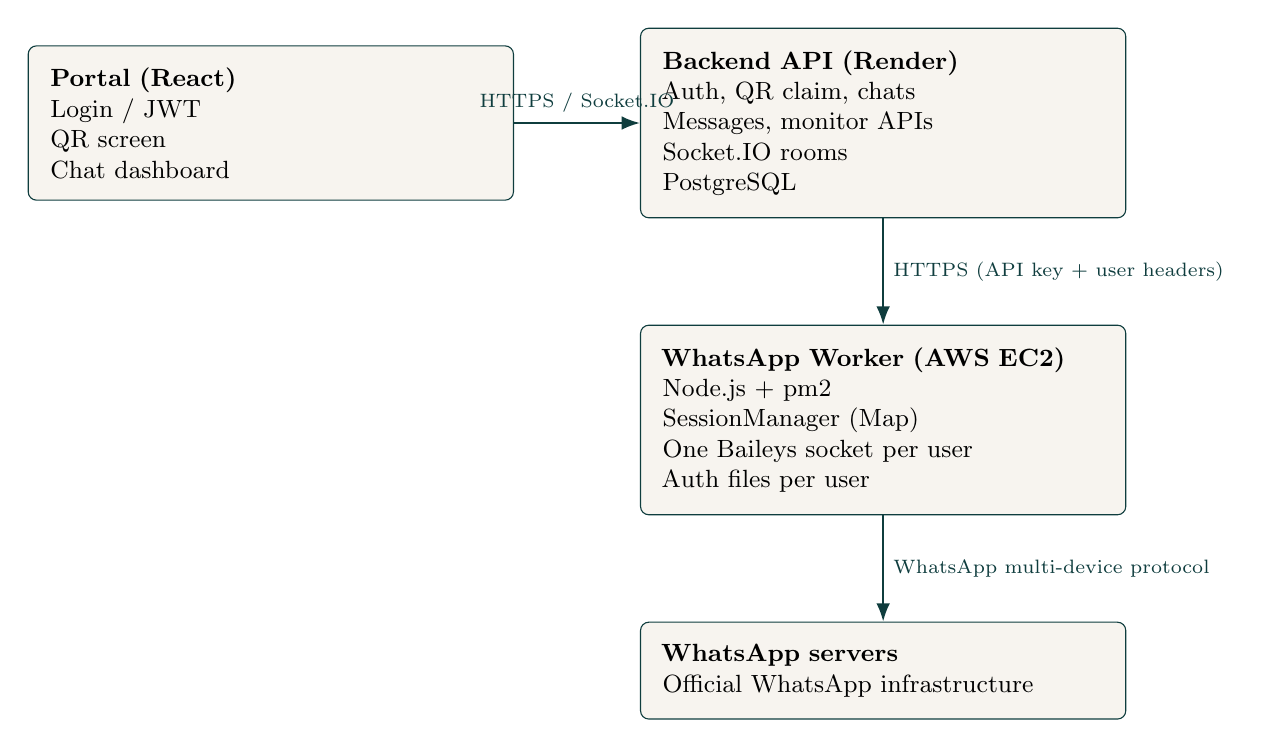
\begin{tikzpicture}[
  font=\small,
  box/.style={draw=brand, rounded corners=3pt, align=left, inner sep=8pt, fill=softbg, text width=5.6cm},
  arrow/.style={-{Latex}, thick, color=brand}
]
\node[box] (portal) {%
  \textbf{Portal (React)}\\
  Login / JWT\\
  QR screen\\
  Chat dashboard};
\node[box, right=1.6cm of portal] (api) {%
  \textbf{Backend API (Render)}\\
  Auth, QR claim, chats\\
  Messages, monitor APIs\\
  Socket.IO rooms\\
  PostgreSQL};
\node[box, below=1.35cm of api] (worker) {%
  \textbf{WhatsApp Worker (AWS EC2)}\\
  Node.js + pm2\\
  SessionManager (Map)\\
  One Baileys socket per user\\
  Auth files per user};
\node[box, below=1.35cm of worker] (wa) {%
  \textbf{WhatsApp servers}\\
  Official WhatsApp infrastructure};

\draw[arrow] (portal.east) -- node[above, font=\scriptsize] {HTTPS / Socket.IO} (api.west);
\draw[arrow] (api.south) -- node[right, font=\scriptsize] {HTTPS (API key + user headers)} (worker.north);
\draw[arrow] (worker.south) -- node[right, font=\scriptsize] {WhatsApp multi-device protocol} (wa.north);
\end{tikzpicture}
\end{center}

\subsection{Component roles}

\begin{tabularx}{\textwidth}{L{3.4cm} L{4.4cm} X}
\toprule
\textbf{Component} & \textbf{Hosting} & \textbf{Responsibility} \\
\midrule
Portal frontend & Client hosting / static app & Login, QR display, monitor chats, view scraped data \\
Backend API & Render & Auth, claims, persistence, realtime events \\
Database & Managed PostgreSQL & Users, chats, messages, link sessions, analysis tables \\
WhatsApp Worker & AWS EC2 & Open/maintain WhatsApp sessions, scrape, push data to backend \\
\bottomrule
\end{tabularx}

\section{Technology stack}

\subsection{WhatsApp Worker (AWS)}

\begin{tabularx}{\textwidth}{L{5.2cm} X}
\toprule
\textbf{Technology} & \textbf{Purpose} \\
\midrule
Node.js 20+ & Runtime \\
Express & Small control API (\texttt{/health}, \texttt{/sessions/...}) \\
\texttt{@whiskeysockets/baileys} & WhatsApp multi-device WebSocket client: open sessions, QR, receive messages \\
\texttt{qrcode} & Convert QR payload to data URL when needed \\
\texttt{pino} & Structured logging \\
\texttt{dotenv} & Environment configuration \\
pm2 & Process manager (keepalive / restart on EC2) \\
Filesystem auth state & \texttt{useMultiFileAuthState} $\rightarrow$ \texttt{sessions/user\_<id>/} \\
\bottomrule
\end{tabularx}

\paragraph{Recommended EC2 sizing (current guidance).}
\begin{itemize}[leftmargin=1.2em]
  \item AMI: Ubuntu 22.04
  \item Instance: \texttt{t3.medium} (2 vCPU / 4~GB) for a small number of concurrent clients
  \item Disk: $\sim$30~GB gp3 for OS, Node, and session auth files
  \item Process: single Node process hosting many in-memory sessions
\end{itemize}

\subsection{Backend API (Render)}

\begin{tabularx}{\textwidth}{L{5.2cm} X}
\toprule
\textbf{Technology} & \textbf{Purpose} \\
\midrule
Node.js + Express & REST API \\
PostgreSQL (\texttt{pg}) & Primary datastore \\
Socket.IO & Realtime QR / connection / chat updates to portal \\
JWT (\texttt{jsonwebtoken}) & Portal authentication \\
\texttt{bcryptjs} & Password hashing \\
\texttt{cors} / \texttt{dotenv} & Cross-origin and configuration \\
\bottomrule
\end{tabularx}

\subsection{Portal frontend}

\begin{tabularx}{\textwidth}{L{5.2cm} X}
\toprule
\textbf{Technology} & \textbf{Purpose} \\
\midrule
React & User interface \\
Socket.IO client & Live QR and connection status \\
REST calls to backend & Claim QR, list chats, monitor, delete, and related APIs \\
\bottomrule
\end{tabularx}

\subsection{What we intentionally do not use in production}

\begin{itemize}[leftmargin=1.2em]
  \item Chrome / Chromium automation (Puppeteer / Playwright) for WhatsApp Web
  \item Browser extensions reading the WhatsApp Web DOM
  \item Selenium-style UI scraping
\end{itemize}

Those approaches are fragile (UI changes break scrapers) and harder to scale. The current design uses \textbf{protocol-level linked-device sessions}.

\section{How WhatsApp sessions are opened on AWS}

\subsection{One portal user = one worker session}

The worker keeps an in-memory map:

\begin{lstlisting}
sessions: Map<userId, SessionState>
\end{lstlisting}

Each \texttt{SessionState} contains:
\begin{itemize}[leftmargin=1.2em]
  \item its own Baileys socket (\texttt{makeWASocket})
  \item auth directory \texttt{sessions/user\_<userId>/}
  \item connection status (\texttt{starting} / \texttt{qr} / \texttt{connected} / \texttt{reconnecting} / \texttt{error})
  \item monitored chat JIDs
  \item message cache / dedupe keys
  \item reconnect timers
\end{itemize}

\textbf{Important:} ``Multiple WhatsApps open at once'' means \textbf{multiple Baileys sockets inside one Node process}, not multiple Chrome tabs.

\subsection{Session start flow (end-to-end)}

\begin{enumerate}[leftmargin=1.4em]
  \item Portal user logs in and opens the WhatsApp connect page.
  \item Frontend calls backend \texttt{POST /api/qr/claim} for that \texttt{userId}.
  \item Backend stores/updates a row in \texttt{whatsapp\_link\_sessions} (\texttt{waiting} or already \texttt{linked}).
  \item Worker polls backend claims (default every $\sim$5 seconds).
  \item For each claimed \texttt{userId}, worker calls \texttt{sessions.start(userId)}.
  \item Worker boots a Baileys socket with that user's auth folder.
  \item If no saved credentials exist, WhatsApp issues a QR.
  \item Worker posts QR to backend (\texttt{/api/qr/...}).
  \item Backend emits Socket.IO events to that user's room (\texttt{user\_<id>}).
  \item Portal shows QR; client scans with WhatsApp mobile app $\rightarrow$ Linked Devices.
  \item On success, worker marks session connected and notifies backend (\texttt{linked}).
  \item Auth credentials are saved under \texttt{sessions/user\_<id>/} so reconnects survive worker restarts.
\end{enumerate}

\subsection{Persistence and restore}

\begin{itemize}[leftmargin=1.2em]
  \item On EC2 reboot / pm2 restart, worker runs \texttt{restoreAll()}.
  \item Any folder \texttt{sessions/user\_<id>/} that contains valid \texttt{creds.json} is restored.
  \item Empty/broken auth folders are skipped or cleared to avoid reconnect storms.
  \item Logout / invalid session clears auth and resets claim to \texttt{waiting} so a fresh QR can be issued.
\end{itemize}

\subsection{Sticky WhatsApp binding (tenant safety)}

Each portal user can be permanently bound to the first successfully linked WhatsApp number (\texttt{bound\_whatsapp\_jid} / \texttt{bound\_whatsapp\_phone}).

If the same portal user later tries to link a \textbf{different} WhatsApp number, backend can reject with \texttt{409 WHATSAPP\_BIND\_MISMATCH}, and the worker logs out / clears that wrong session.

This prevents accidental (or intentional) switching of a tenant's linked number after onboarding.

\section{How scraping works (without extensions)}

Scraping is \textbf{event-driven} from Baileys WhatsApp events, then filtered and stored.

\subsection{Chat list sync}

When a session connects, WhatsApp sends chat metadata via events such as:
\begin{itemize}[leftmargin=1.2em]
  \item \texttt{messaging-history.set}
  \item \texttt{chats.upsert} / \texttt{chats.update}
\end{itemize}

Worker normalizes each chat to \texttt{\{ id: jid, name \}} and posts contacts/chats to the backend for that \texttt{userId}. Result: portal can show the user's chat list.

\subsection{Monitored-chat filter (important product rule)}

The worker does \textbf{not} continuously dump every message from every chat into long-term scraping storage by default.

It periodically fetches monitored chats from backend:

\begin{lstlisting}
GET /api/scraped-chats/monitored?userId=...
\end{lstlisting}

Only JIDs in that monitored set have messages posted as scraped content.

\subsection{Historical scrape (when a chat is newly monitored)}

For each newly monitored chat, worker runs a history sync:
\begin{enumerate}[leftmargin=1.4em]
  \item Flush any already-cached messages for that chat.
  \item Use Baileys \texttt{fetchMessageHistory(...)} to page backwards (batches of $\sim$50).
  \item Incoming history batches arrive on \texttt{messaging-history.set}.
  \item Worker posts text messages to backend until configured limit (default $\sim$500) or no more pages.
\end{enumerate}

\subsection{Live scrape (ongoing)}

On \texttt{messages.upsert}:
\begin{enumerate}[leftmargin=1.4em]
  \item Cache message.
  \item Ignore non-monitored chats.
  \item Deduplicate by WhatsApp message key.
  \item Extract text content and \texttt{fromMe} (outgoing vs incoming).
  \item POST to backend in chunks (\texttt{postMessages}).
\end{enumerate}

\subsection{What is extracted today}

Typically text-bearing content: plain text, captions on media, and related extended text fields. Non-text media-only messages may be skipped by current extractors.

Each stored message includes roughly: \texttt{chat\_jid}, \texttt{sender}, \texttt{timestamp}, \texttt{message}, \texttt{from\_me}, and \texttt{user\_id} (tenant).

\section{Data model (conceptual)}

\begin{tabularx}{\textwidth}{L{5.6cm} X}
\toprule
\textbf{Table} & \textbf{Purpose} \\
\midrule
\texttt{users} & Portal accounts; optional sticky WhatsApp bind fields \\
\texttt{whatsapp\_link\_sessions} & Claim/link state per user (\texttt{waiting} / \texttt{linked}) \\
\texttt{whatsapp\_chats} & Chat list per user (\texttt{jid}, name, \texttt{is\_monitored}) \\
\texttt{whatsapp\_messages} & Scraped messages per user \\
\texttt{normalized\_messages} / related AI tables & Downstream analysis (optional) \\
\bottomrule
\end{tabularx}

\vspace{8pt}
Isolation principle: \textbf{every chat/message row is scoped by \texttt{user\_id}}. Additional APIs include monitor toggles and delete endpoints for selected messages/chats.

\section{How the WhatsApp Worker works today}

\subsection{Process model}

\begin{itemize}[leftmargin=1.2em]
  \item One Node process (\texttt{whatsapp-worker}) managed by pm2.
  \item Internal HTTP server (default port \texttt{4100}) for health/control.
  \item Protected by \texttt{WORKER\_API\_KEY} (\texttt{x-api-key}).
  \item Outbound calls to Render backend with user scoping headers.
\end{itemize}

\subsection{Claim polling loop}

Every few seconds the worker:
\begin{enumerate}[leftmargin=1.4em]
  \item Reads active claims from backend.
  \item Starts sessions for claimed users (\texttt{waiting} or \texttt{linked}).
  \item Skips admin / \texttt{userId=1} as a WhatsApp client by policy.
  \item Stops sessions that no longer have claims (with safeguards for healthy connected sessions during transient claim gaps).
\end{enumerate}

\subsection{Connection lifecycle per user}

\begin{lstlisting}
start(userId)
  -> boot Baileys socket
  -> QR? post QR to backend
  -> open? mark linked, sync chats, refresh monitored set
  -> close? reconnect with backoff OR clear auth if logged out
\end{lstlisting}

\subsection{Why this scales better than extensions}

\begin{tabularx}{\textwidth}{X X}
\toprule
\textbf{Extension model} & \textbf{Worker model} \\
\midrule
Browser + WhatsApp Web UI & Protocol client \\
DOM selectors break often & Event APIs (\texttt{messages.upsert}, history fetch) \\
Hard to run many profiles headlessly & Many sockets in one process \\
Laptop-bound & Centralized on AWS \\
\bottomrule
\end{tabularx}

\section{Scaling to $\sim$1{,}000 WhatsApp sessions --- IP / ban risk}

\subsection{Direct answer}

\riskbox{Yes --- putting $\sim$1{,}000 WhatsApp linked sessions on a single AWS public IP is high risk and can trigger WhatsApp anti-abuse systems. This can result in client WhatsApp accounts being disconnected or restricted.}

WhatsApp does not need a special ``scraper detector'' unique to our code. From their side, they already see:
\begin{itemize}[leftmargin=1.2em]
  \item many independent multi-device connections
  \item coming from the \textbf{same IP / same cloud ASN (Amazon)}
  \item often with similar client fingerprints (Baileys / linked-device patterns)
  \item potentially abnormal volume of history sync / connection churn
\end{itemize}

That pattern is commonly associated with spam, bulk automation, or account farming. WhatsApp can respond with:
\begin{itemize}[leftmargin=1.2em]
  \item connection failures before/during QR
  \item sudden disconnects
  \item ``logged out'' / device removed
  \item temporary or longer blocks on numbers or IP ranges
\end{itemize}

\textbf{Same-server, same-IP mass linking is a real ban/closure risk for client WhatsApp accounts.} This is one of the most important operational risks in the architecture.

\subsection{What WhatsApp can observe}

Even without us ``notifying'' them explicitly, each session is a normal connection to WhatsApp servers. At scale they can correlate:

\begin{tabularx}{\textwidth}{L{5.4cm} X}
\toprule
\textbf{Signal} & \textbf{Risk if thousands share one EC2 IP} \\
\midrule
Source IP / ASN & Very high (datacenter IP concentration) \\
Concurrent linked devices from one IP & Very high \\
Repeated QR / reconnect storms & High \\
Aggressive history fetch patterns & Medium--high \\
Unofficial client fingerprints & Medium--high (Baileys is not an official WhatsApp Business API) \\
\bottomrule
\end{tabularx}

\subsection{Practical guidance}

\begin{tabularx}{\textwidth}{L{6.2cm} X}
\toprule
\textbf{Concurrent sessions on one public IP} & \textbf{Expected risk} \\
\midrule
Few (pilot / small team) & Manageable, still not zero (cloud IP risk exists) \\
Tens & Elevated; monitor disconnects carefully \\
Hundreds--1{,}000 on one IP & \textbf{Not recommended} --- ban/closure risk becomes likely \\
\bottomrule
\end{tabularx}

\subsection{Required direction if the product must support $\sim$1{,}000 clients}

To reduce correlation risk, architecture must evolve beyond ``one EC2 IP for everyone'':

\begin{enumerate}[leftmargin=1.4em]
  \item \textbf{IP isolation.} Prefer residential / mobile proxy or dedicated egress IP per session or small session groups. Avoid funneling all sockets out one AWS elastic IP.
  \item \textbf{Horizontal workers.} Multiple worker nodes across regions/providers. Shard users across workers (\texttt{userId} ranges / assignment table).
  \item \textbf{Rate limiting and soft start.} Stagger QR starts, history sync, reconnects. Cap concurrent history pagination.
  \item \textbf{Health / ban detection.} Auto-pause users showing repeated auth failures. Alert ops before mass reconnect loops amplify risk.
  \item \textbf{Official API path (long-term compliance).} For enterprise-grade legality/stability, evaluate WhatsApp Cloud API / BSP where the use-case fits. Baileys-based linked-device automation is powerful but is \textbf{not} an officially supported WhatsApp business channel and carries ToS / enforcement risk.
\end{enumerate}

\subsection{Product statement}

\begin{quote}
The current worker successfully supports multi-user WhatsApp linking and scraping on AWS for a \textbf{controlled} number of concurrent sessions.

Scaling to $\sim$1{,}000 simultaneous WhatsApp connections from a \textbf{single AWS IP} is \textbf{not safe} from an anti-abuse perspective.

A production scale-out plan must include \textbf{egress IP isolation} (proxies / multiple exit nodes) and \textbf{sharded workers}; otherwise client numbers can be disconnected or restricted by WhatsApp.
\end{quote}

\section{Security posture and known gaps}

This section is intentionally candid for client transparency and remediation planning.

\subsection{Architectural / platform risks}

\begin{tabularx}{\textwidth}{L{4.4cm} L{3.2cm} X}
\toprule
\textbf{Item} & \textbf{Severity} & \textbf{Notes} \\
\midrule
Unofficial WhatsApp client (Baileys) & High (compliance) & Not WhatsApp-official; ToS and enforcement risk \\
Session auth files on disk & High & \texttt{creds.json} = account link secrets; disk compromise = session theft \\
Cloud IP reputation & High at scale & AWS IPs are more scrutinized than residential \\
Single worker host & Medium--High & Compromise of one box affects many linked sessions \\
\bottomrule
\end{tabularx}

\subsection{Application security gaps / residual risks}

\begin{tabularx}{\textwidth}{L{4.2cm} L{2.8cm} X}
\toprule
\textbf{Item} & \textbf{Severity} & \textbf{Detail / recommendation} \\
\midrule
Worker control plane exposure & High if public & Port \texttt{4100} must not be open to the world; restrict security group to admin IP/VPN; keep strong \texttt{WORKER\_API\_KEY} \\
Default/weak secrets & High if unchanged & Ensure strong \texttt{WORKER\_API\_KEY}, \texttt{JWT\_SECRET}, and DB credentials in all environments \\
Tenant spoofing via headers & Medium--High & Worker flows may use \texttt{x-user-id} / force headers; untrusted clients must not impersonate other tenants \\
Multi-tenant isolation bugs & High impact & Any missed \texttt{user\_id} filter in queries = cross-tenant data leak \\
Socket room joining & Medium & Users must only join their own \texttt{user\_<id>} room \\
Auth credential backup & Medium & Session folders may be copied in AMI snapshots/backups without encryption controls \\
No hardware-backed secret store & Medium & Prefer KMS/Secrets Manager + encrypted volume for session store at scale \\
Delete/monitor API authorization & Medium & Always enforce authenticated user scope server-side (never trust body \texttt{userId} alone) \\
Logging of message content & Low--Medium & Logs may contain PII; define retention and redaction \\
Dependency risk & Medium & Baileys/ecosystem changes can break linking overnight \\
\bottomrule
\end{tabularx}

\subsection{Data protection considerations}

\begin{itemize}[leftmargin=1.2em]
  \item Scraped chats are private communications; treat as sensitive personal data.
  \item Define retention, export, and deletion policies (delete APIs exist for selected chats/messages).
  \item Restrict who (admin vs client) can view which tenant data.
  \item Encrypt in transit (HTTPS) everywhere; plan encryption at rest for DB and session volumes.
\end{itemize}

\subsection{Recommended security hardening roadmap}

\begin{enumerate}[leftmargin=1.4em]
  \item Private networking between worker and backend (VPN / Tailscale / private ingress).
  \item Rotate and vault all secrets.
  \item Encrypt EC2 disks; restrict IAM; no public worker ports.
  \item Strict tenant authorization middleware on every read/write route.
  \item Audit logging for claim/link/monitor/delete actions.
  \item Proxy-per-session (or per small cohort) before large-scale rollout.
  \item Penetration test focused on tenant isolation and worker API.
\end{enumerate}

\section{Operational characteristics}

\subsection{Current operating model}

\begin{itemize}[leftmargin=1.2em]
  \item Worker always-on (pm2)
  \item Backend always-on (Render)
  \item Sessions restored from disk after restart
  \item Monitored list refreshed on an interval
  \item Reconnect with backoff-style delays on disconnect
\end{itemize}

\subsection{Approximate infrastructure cost (ballpark)}

For a small deployment (not 1{,}000 sessions):

\begin{tabularx}{\textwidth}{X L{4.2cm}}
\toprule
\textbf{Item} & \textbf{Monthly ballpark} \\
\midrule
EC2 \texttt{t3.medium} + disk + light transfer & $\sim$\$35--45 \\
Render backend & $\sim$\$0--25 \\
Managed Postgres (small) & $\sim$\$0--15 \\
\textbf{Typical small total} & \textbf{$\sim$\$40--80} \\
\bottomrule
\end{tabularx}

\vspace{8pt}
At 1{,}000 sessions, cost is dominated not only by CPU/RAM, but by \textbf{proxy/IP isolation strategy} (often larger than the EC2 bill).

\subsection{Capacity note}

A single \texttt{t3.medium} is suitable for a \textbf{small} concurrent session count. 1{,}000 concurrent Baileys sockets generally requires multiple larger workers, careful memory planning, and IP sharding --- not one small instance.

\section{End-to-end user journey (as implemented)}

\begin{enumerate}[leftmargin=1.4em]
  \item Client logs into portal.
  \item Portal claims QR session for that user.
  \item Worker starts Baileys session for that user on AWS.
  \item QR appears in portal; client scans on phone.
  \item WhatsApp marks device linked; worker persists credentials.
  \item Chat list appears in portal.
  \item Client selects chats to monitor.
  \item Worker syncs history and continues live message ingestion.
  \item Messages appear in portal DB views / dashboards.
  \item Client can delete selected messages/chats via delete API.
\end{enumerate}

\section{Key libraries and protocols}

\subsection{Worker}

\begin{itemize}[leftmargin=1.2em]
  \item \texttt{@whiskeysockets/baileys} --- WhatsApp multi-device protocol client
  \item \texttt{useMultiFileAuthState} --- persist Signal/WhatsApp auth keys to disk
  \item \texttt{makeWASocket} --- open one socket per tenant
  \item Events used: \texttt{connection.update}, \texttt{creds.update}, \texttt{messaging-history.set}, \texttt{chats.upsert}, \texttt{chats.update}, \texttt{messages.upsert}
  \item History API: \texttt{fetchMessageHistory}
\end{itemize}

\subsection{Backend}

\begin{itemize}[leftmargin=1.2em]
  \item Express routes for QR claim/status, scraped chats/messages, monitor, delete
  \item Socket.IO rooms \texttt{user\_<id>} for realtime UX
  \item PostgreSQL uniqueness constraints for chats/messages per user
\end{itemize}

\section{Conclusions}

\begin{enumerate}[leftmargin=1.4em]
  \item \textbf{How we open WhatsApp on AWS:} one Baileys linked-device session per portal user inside a Node worker on EC2, with per-user auth folders and claim-driven auto-start.
  \item \textbf{How we scrape:} protocol events + monitored-chat filter + history pagination + live upserts; \textbf{no Chrome extensions} in production.
  \item \textbf{Tech stack:} Node.js, Baileys, Express, PostgreSQL, Socket.IO, React, pm2, AWS EC2, Render.
  \item \textbf{Scale warning:} $\sim$1{,}000 WhatsApps on \textbf{one AWS IP} is likely to attract WhatsApp anti-abuse actions; client numbers can be disconnected/restricted. Scale-out requires IP isolation and sharded workers.
  \item \textbf{Security:} a functional multi-tenant architecture exists, but production hardening (secrets, private networking, encrypted session storage, strict tenant auth, proxy strategy) should be treated as mandatory before large-scale commercial rollout.
\end{enumerate}

\section{Appendix --- glossary}

\begin{tabularx}{\textwidth}{L{3.6cm} X}
\toprule
\textbf{Term} & \textbf{Meaning} \\
\midrule
JID & WhatsApp identifier for a chat/user (e.g.\ \texttt{number@s.whatsapp.net}, group \texttt{@g.us}) \\
Baileys & Open-source WhatsApp multi-device client library \\
Claim & Backend reservation that a portal \texttt{userId} should have an active worker session \\
Monitored chat & Chat selected by client for message scraping \\
Linked device & Phone-authorized companion session (worker acts as one) \\
Sticky bind & Portal user permanently associated with first linked WhatsApp number \\
\bottomrule
\end{tabularx}

\vspace{1.2cm}
{\small\textit{This document describes the implemented technical system and known risks for planning, client communication, and scale/security roadmap decisions.}}

\end{document}
